\chapter{Технологический раздел}
\label{cha:impl}

%В данном разделе проанализированы и выбраны: язык программирования, инструменты для создания пользовательского интерфейса, выбрана среда разработки и другие инструменты для реализации проекта.

%Проверить все старое
\section{Основные инструменты, используемые для реализации}

\noindent\textbf{Язык программирования C++.}

C++ -- язык программирования общего назначения с уклоном в сторону системного программирования \cite{Cpp}

Данный язык, достаточно популярен и широко распространен, кроме этого, он имеет ряд плюсов, описанных ниже:

\begin{itemize}
	\item высокая производительность: язык спроектирован так, чтобы дать программисту максимальный контроль над всеми аспектами структуры и порядка исполнения программы; один из базовых принципов C++ «не платишь за то, что не используешь» то есть ни одна из языковых возможностей, приводящая к дополнительным накладным расходам, не является обязательной для использования; имеется возможность работы с памятью на низком уровне;
	\item кроссплатформенность: стандарт языка C++ накладывает минимальные требования на ЭВМ для запуска скомпилированных программ;
	\item поддержка различных стилей программирования: традиционное императивное программирование (структурное, объектно-ориентированное), обобщенное программирование, функциональное программирование, порождающее метапрограммирование.
\end{itemize}

Исходя из вышеперечисленных плюсов, очевиден выбор данного языка программирования для реализации поставленной задачи. %ToDo?

%\newpage
\noindent\textbf{Кроссплатформенный фреймворк Qt.}

Для реализации данного проекта, необходима была библиотека, упрощающая создание интерфейса.
%На примете были Qt и MFC. Чтобы сделать выбор, пришлось их сравнить. 

Qt – кроссплатформенный фреймворк для разработки программного обеспечения на языке программирования C++. Есть также «привязки» ко многим другим языкам программирования: Python — PyQt, PySide; Ruby — QtRuby; Java — Qt Jambi; PHP — PHP-Qt и другие. Поддерживаемые платформы включают Linux, OS X, Windows, VxWorks, QNX, Android, iOS, BlackBerry, ОС Sailfish и другие \cite{Qt}.

Qt позволяет запускать написанное с его помощью программное обеспечение в большинстве современных операционных систем путем простой компиляции программы для каждой системы без изменения исходного кода (кроссплатформенность). Включает в себя все основные классы, которые могут потребоваться при разработке прикладного программного обеспечения, начиная от элементов графического интерфейса и заканчивая классами для работы с сетью, базами данных и XML. Является полностью объектно-ориентированным, расширяемым и поддерживающим технику компонентного программирования.

Комплектуется визуальной средой разработки графического интерфейса Qt Designer, позволяющей создавать диалоги и формы.

Также существует возможность расширения привычной функциональности виджетов, связанной с размещением их на экране, отображением, перерисовкой при изменении размеров окна.

Мета-объектная система — часть ядра фреймворка для поддержки в С++ таких возможностей, как сигналы и слоты для коммуникации между объектами в режиме реального времени и динамических свойств системы.

Одним из преимуществ проекта Qt является наличие качественной документации. Статьи документации снабжены большим количеством примеров. Исходный код самой библиотеки хорошо форматирован, подробно комментирован, что также упрощает изучение Qt.

Отличительная особенность — использование мета-объектного компилятора — предварительной системы обработки исходного кода. Расширение возможностей обеспечивается системой плагинов, которые возможно размещать непосредственно в панели визуального редактора. Но минусом получается то, что код написанный с помощью Qt нельзя скомпилировать на другом компьютере без установки фреймворка.

%Microsoft Foundation Classes – библиотека на языке C++, разработанная Microsoft и призванная облегчить разработку GUI-приложений для Microsoft Windows путём использования богатого набора библиотечных классов.
%Во-первых, если сравнивать только работу с GUI, то данная библиотека работает только под Windows, то есть ни о какой кроссплатформенности речи не идёт. Но не стоит забывать о том, что Qt в отличии от MFC имеет множество других полезных классов. Во-вторых, если же в MFC создать каркас приложения без дизайнера достаточно сложно, то в Qt это зачастую даже намного удобнее и проще.

%Поскольку функционал Qt намного шире, то для реализации проекта был выбран именно фреймворк Qt.

Вывод про кроссплатформенность и многофункциональность.

\noindent\textbf{Среда разработки Qt creator.}

Qt Creator (ранее известная под кодовым названием Greenhouse) — кроссплатформенная свободная IDE для языков С, С++ и QML. Разработана Trolltech (Digia) для работы с фреймворком Qt. Включает в себя графический интерфейс отладчика и визуальные средства разработки интерфейса как с использованием QtWidgets, так и QML. Поддерживаемые компиляторы: GCC, Clang, MinGW, MSVC, Linux ICC, GCCE, RVCT, WINSCW.

Основная задача Qt Creator — упростить разработку приложения с помощью фреймворка Qt на разных платформах. Поэтому для работы с данной библиотекой был выбран именно он.

\noindent\textbf{Система версионного контроля git.}

Для хранения исходников используется система Git (на портале github.com), т.к. это крупнейший веб-сервис для хостинга IT-проектов и их совместной разработки. %Нужно ли?

%Добавить про SQLite
\noindent\textbf{СУБД SQLite}

Для работы с базой данных была выбрана СУБД SQLite, т.к. она не работает в режиме сервера-клиента, а встраивается непосредственно в приложение. Это означает, что вся база данных хранится в одном файле, который обрабатывается непосредственно приложением.

\section{Входные и выходные данные}
%Что тут писать, описать вид логов нанокад?
Данная программа разрабатывается для анализа логов САПР NanoCAD, которые имеют следующий вид:
% (рис. \ref{NanoCAD_logs}):

%Пример входного файла, см в приложении
%\begin{figure}[h!] %Как сделать скрин в векторе или более качественно показать логи?
%	\centering
%	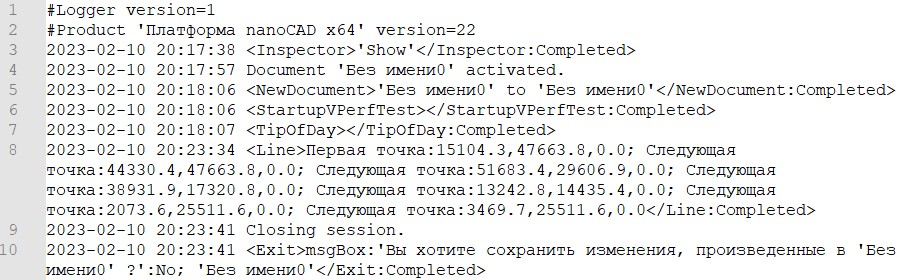
\includegraphics[width=1\textwidth]{inc/img/logs2.jpg}
%	\caption{Пример логов NanoCAD}
%	\label{NanoCAD_logs}
%\end{figure}

% Листинг?
%\begin{lstlisting}[caption={Пример логов NanoCAD}, label={logs2}]
%	#Logger version=1
%	#Product 'Платформа nanoCAD x64' version=22
%	2023-02-10 20:17:38 <Inspector>'Show'</Inspector:Completed>
%	2023-02-10 20:17:57 Document 'Без имени0' activated.
%	2023-02-10 20:18:06 <NewDocument>'Без имени0' to 'Без имени0'</NewDocument:Completed>
%	2023-02-10 20:18:06 <StartupVPerfTest></StartupVPerfTest:Completed>
%	2023-02-10 20:18:07 <TipOfDay></TipOfDay:Completed>
%	2023-02-10 20:23:34 <Line>Первая точка:15104.3,47663.8,0.0; Следующая точка:44330.4,47663.8,0.0; Следующая точка:51683.4,29606.9,0.0; Следующая точка:38931.9,17320.8,0.0; Следующая точка:13242.8,14435.4,0.0; Следующая точка:2073.6,25511.6,0.0; Следующая точка:3469.7,25511.6,0.0</Line:Completed>
%	2023-02-10 20:23:41 Closing session.
%	2023-02-10 20:23:41 <Exit>msgBox:'Вы хотите сохранить изменения, произведенные в 'Без имени0' ?':No; 'Без имени0'</Exit:Completed>
%\end{lstlisting}

Каждая строчка, содержащая действие, начинается с даты и времени выполнения. Начало каждой команды обозначается ее названием, заключенной в символы '<' и '>'. Завершение команды обозначается аналогично, но перед названием команды добавляется символ '/'. Пример входного файла, см в приложении Б. 

Также поддерживается считывание обезличенных логов, которые не содержат информации о параметрах команд, включая время выполнения. В таком случае время выполнения для каждой команды в сессии будет выставлено автоматически, начиная с 0, увеличивая это значения на 1 для каждой следующей команды.

Кроме этого на вход программе подаются минимальный уровень поддержки, а также минимальный и максимальный разрывы между командами.

%STOPPED HERE
%Нужно в РПЗ перевести lift? Нужно ли чтобы в программе все было на русском?
На выходе программа выдает часто встречающиеся последовательности команд, их уровни поддержки и lift'а.
%lift показывает отношение <<зависимости>> команд в последовательности к их <<независимости>>. %lift - коэф зависимости
lift показывает насколько команды в последовательности зависят друг от друга. 
Считается как отношение поддержки последовательности к произведению поддержек всех подпоследовательностей состоящих из 1 команды. Если значение lift <= 1, значит зависимости нету. Если же lift > 1, то зависимость есть. Чем больше единицы, тем вероятней то, что эти команды использовались вместе.
% Из аналита:
%На вход программе подаются информация о выполненных командах (логи), минимальный уровень поддержки, минимальный и максимальный разрывы между командами. Используя методы поиска последовательных шаблонов система определяет часто встречающиеся последовательности команд.

\section{Реализация}
%Разработать программное обеспечение, реализующее описанный метод
%Что тут писать?
За преобразование логов из текста в таблицу базы данных отвечает класс \textit{LogReader}.
%реализованный по паттерну Singleton.
Он может считать все файлы с расширением *.log в выбранной директории и её поддиректориях, записывая все команды в таблицу logs для выбранной на текущий момент базы данных. Также можно указать, нужно ли учитывать завершение команды как отдельное действие, если она началась и закончилась одновременно.

За взаимодействие с базами данных отвечает класс \textit{DataBase}.
%, также реализованный в соответствии с паттерном Singleton.
Данный класс позволяет создавать базы данных,
%(которые являются файлами с расширением *.sqlite),
переключаться между ними и как записывать в них необходимые данные, так и считывать их.

За реализацию разрабатываемого метода отвечает
%отдельный класс.
класс \textit{GSP}. %Переименовать класс? Calculator
Он хранит входные параметры алгоритма а также необходимые для работы данные и последний полученный результат.
%Добавить ссылку на приложение, где показаны .h файлы этих классов

%Нужно ли писать про UI?
%Основное взаимодействия пользователя с программой производится через главное окно.
Пользовательский интерфейс позволяет выбирать и просматривать базу данных, считывать в базу данных логи из выбранной директории, задавать режимы считывания логов, задавать параметры самого алгоритма, запускать его для текущей базы данных и наблюдать результат как в основном, так и отдельном окне.
%На рисунках \ref{interface1}-\ref{interface2} показан интерфейс программы.
%Подробно про все окно
% Результат работы программы


\section{Примеры работы программы}

На рисунке \ref{interface1} показан интерфейс программы и начало базы данных используемой в последующих примерах.
Для простоты и наглядности анализировались логи, где большинство сессий подряд повторялись одинаковые действия. На рисунке \ref{example1} приведен пример работы программы без учета последовательностей с повторяющимися по две или более подряд командами. На рисунке \ref{example2} показан результат анализа тех же логов, но с учетом последовательностей с повторяющимися командами.

%Перенести в приложение
\newpage
\begin{figure}[h!]
	\centering
	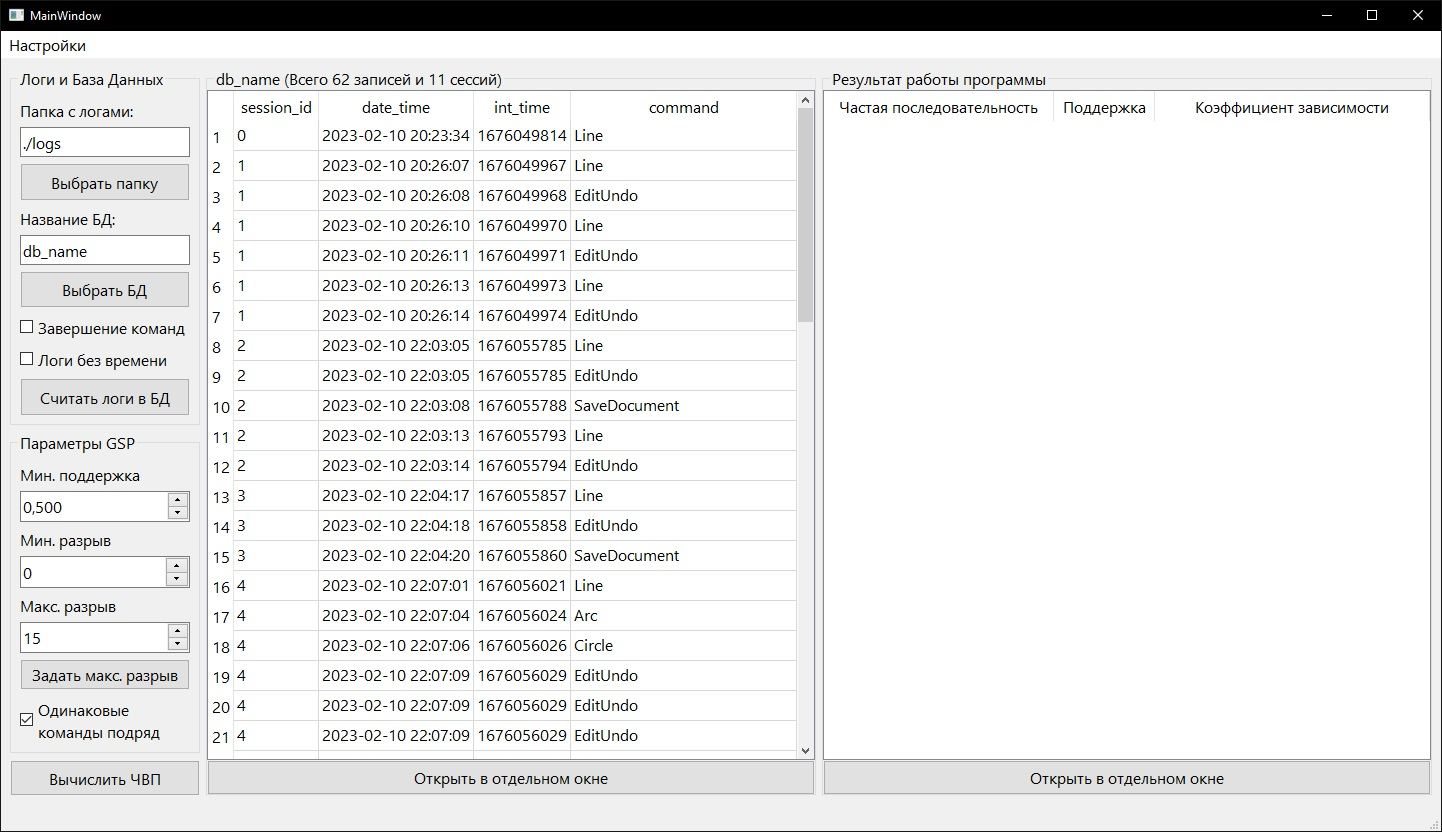
\includegraphics[width=1\textwidth]{inc/img/interface1.jpg}
	\caption{Интерфейс программы 1}
	\label{interface1}
\end{figure}

%\begin{figure}[h!]
%\centering
%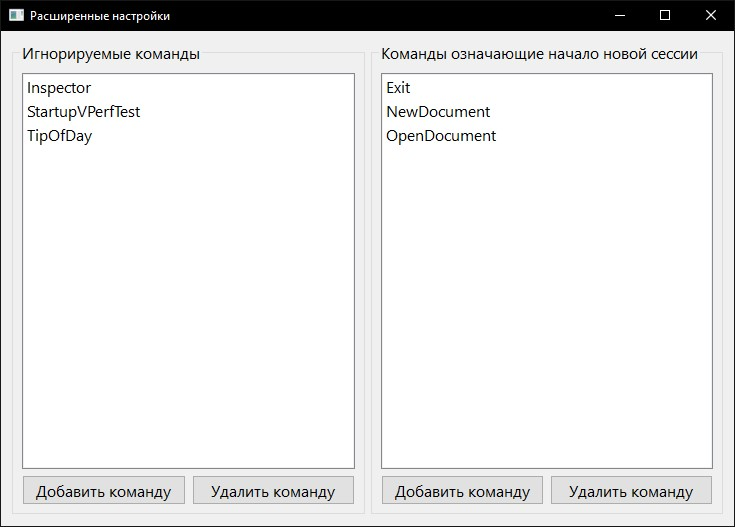
\includegraphics[width=1\textwidth]{inc/img/interface2.jpg}
%\caption{Интерфейс программы 2}
%\label{interface2}
%\end{figure}

\newpage
\begin{figure}[h!] %Как сделать скрин в векторе или более качественно показать пример работы программы?
	\centering
	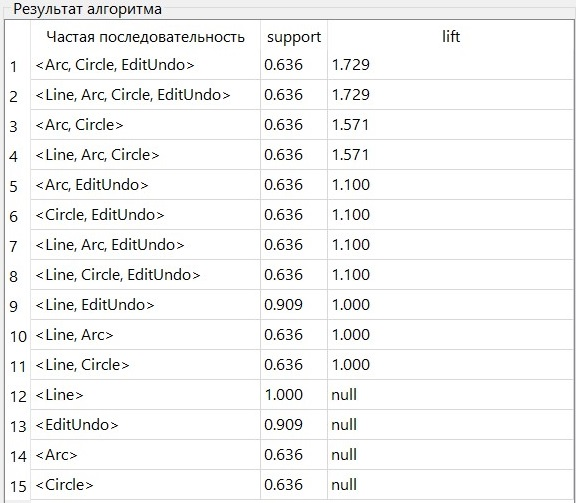
\includegraphics[width=1\textwidth]{inc/img/example1.jpg}
	\caption{Пример работы программы 2}
	\label{example1}
\end{figure}

\newpage
\begin{figure}[h!]
	\centering
	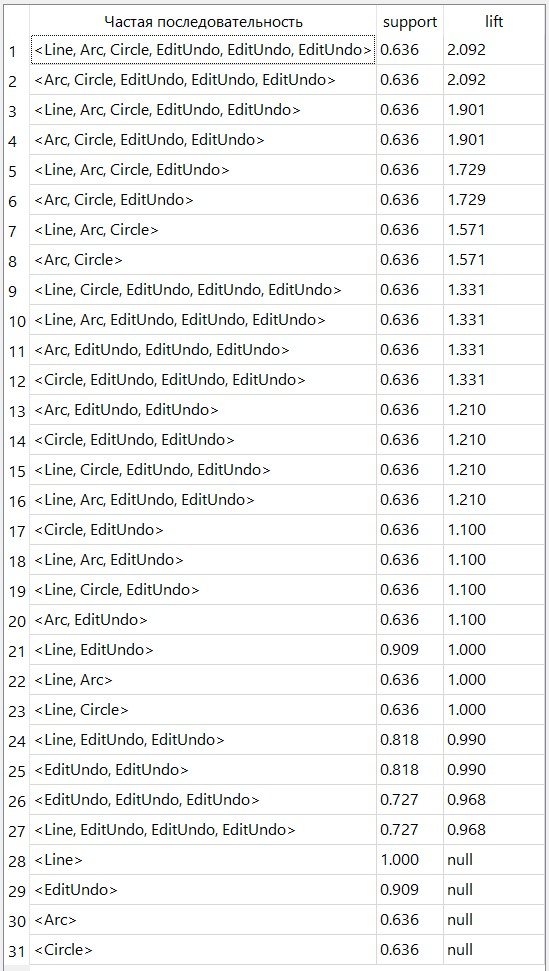
\includegraphics[width=0.8\textwidth]{inc/img/example2.jpg}
	\caption{Пример работы программы 2}
	\label{example2}
\end{figure}

\newpage
\section*{Вывод из технологического раздела}
В данном разделе был обоснован выбор основных инструментов, используемых для реализации, описан формат входных и выходных данных, разработано программное обеспечение, реализующее описанный метод и приведены примеры работы программы.